\section{Object-orientation in finite element analysis}
\label{sec:ovl}

Almost all numerical methods eventually have to deal with the
solution of algebraic equation systems. The basic algorithms for
the discretization of partial differential equations (PDEs)
resulting from the initial-boundary-value-problems (IBVPs) of
continuum mechanics can be generalized in principle as follows:
time discretization, calculation of problem-specific node (finite
difference method - FDM), element (finite element method - FEM),
volume (finite volume method - FVM) contributions, incorporating
initial and boundary conditions, assembling and solving the resulting
equation system. For non-linear problems iteration schemes, such
as Picard or Newton methods, have to be used.

The general solution algorithm for the finite element method is
given in Table \ref{tab:alg1}.

\newpage

%.........................................................................
\rule{\textwidth}{0.25mm}
\begin{enumerate}
  \item Domain \rev{discretization} ( i.e. mesh generation): Creation of individual
geometric elements (e.g. triangles, tetrahedra) and their
topological relationships (mesh topology).
  \item Local element assembly: Depending on PDE type (section
\ref{sec:fem}) all element matrices and vectors have to be
computed. The element integration requires geometric operations
such as interpolation with shape functions, calculation of inverse
Jacobians and determinants. Additionally material functions have
to be computed in Gauss points. Material functions can depend on
field variables.
  \begin{itemize}
    \item Geometric element operations (shape functions, Jacobian),
    \item Material parameter calculation at Gauss points,
  \end{itemize}
  \item Global assembly of the algebraic equation $\mathbf{Ax=b}$: The local element
  entries are assembled into the global system matrix $\mathbf A$ and global
  RHS vector $\mathbf b$. The equations systems is established after \rev{incorporating} boundary conditions and source/sink terms.

  \begin{itemize}
    \item Assembly of system matrix $\mathbf A$ (including incorporation of boundary
    conditions),
    \item Assembly of RHS vector $\mathbf b$ (including incorporation of source/sink
    terms),
  \end{itemize}
  \item Solving the system equations,
  \item Iterative methods to handle non-linearities,
  \item Iterative methods to handle couplings (partitioned and monolithic schemes).
\end{enumerate}
\rule{\textwidth}{0.25mm}
\begin{table}[H]
\begin{tabular}{c}
\end{tabular}
 \caption{General solution procedure of the finite element method}
 \label{tab:alg1}
\end{table}

%.........................................................................
The implementation of the general solution algorithm for multi-field
IBVPs according to Table \ref{tab:alg1} is illustrated in Fig.
\ref{fig:alg}. The time loop represents time discretization. Within
the time loop, specified physical processes (e.g. flow, transport,
deformation) are solved using the finite element method (left box).
The solution procedure of each process is unique (middle box). The
basic part is the calculation and assembly of element contribution
(right box).

%.........................................................................
Based on above described general solution algorithm for
multi-field IBVPs, the fundamental concept of object-orientation
in finite element analysis is the generalization of
\begin{itemize}
    \item Process (PCS) types (section \ref{sec:pcs}),
    \item Equation (PDE) types (section \ref{sec:pde}),
    \item Element (ELE) types (section \ref{sec:ele}).
\end{itemize}

\begin{figure}[htb!]
\centering
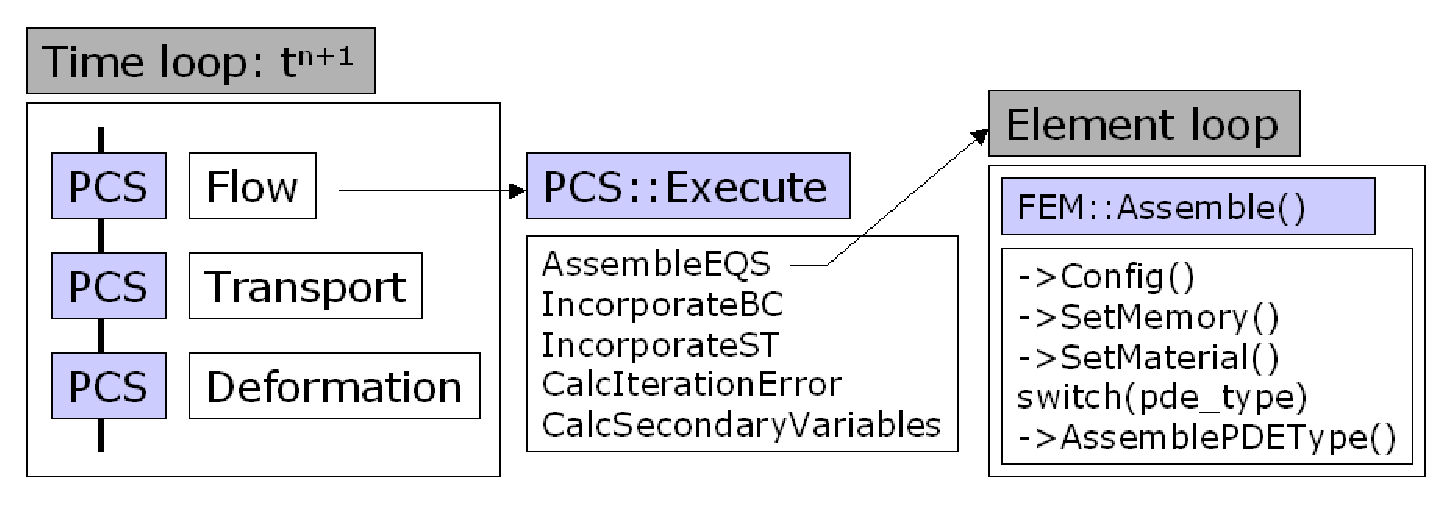
\includegraphics[scale=0.45]{figures/algorithm.eps}
\caption{Implementation of solution algorithm} \label{fig:alg}
\end{figure}

%---
\subsection{Process (PCS) types}
\label{sec:pcs}

The central idea behind object-orientation of processes is that the
basic steps of the solution procedure: calculation of element
contributions, assembly of equation system (including treatment of
boundary conditions and source terms), solution of the equations
system, linearization methods and calculation of secondary variables, 
are independent of the specific problem (e.g. flow,
transport, deformation processes) \cite{{KolBau:04},{geosys}}. The
process (PCS) class provides basic methods in order to solve a PDE
in a very general way. The central part of the PCS object is the
member function \texttt{PCS::Execute()} (Fig. \ref{fig:alg}, middle
box) conducting these basic steps. Specific properties of the
mechanical problem, such as PDE type, primary and secondary
variables and material functions, are assigned during process
configuration (member function \texttt{PCS::Config()}). In order to
configure PCS instances we take advantage of polymorphism.

Fig. \ref{fig:pcs} illustrates the object-orientation of PCS types 
for the solution of IBVPs. The PCS object was designed to manage the 
complete solution algorithm in order to build the global equation 
system (EQS). In fact, the PCS object 'only' administrates 
references to geometric (GEO) objects (points, polylines, surfaces, 
volumes); MSH objects (mesh nodes, elements and mesh topology), 
node-related data such as initial (IC) and boundary (BC) conditions 
as well as source terms (ST); material data of porous media (fluid 
(MFP), solid (MSP), medium (MMP) and chemical (MCP) properties); 
parameters of the different numerical methods (NUM). PCS instances 
have 'only' pointers to the related objects as members. \rev{Objects 
IC, BC and ST have pointers to object GEO to specify geometrical 
entities, which are managed by PCS to find element nodes on them. 
The values in IC and BC and ST are assigned to element nodes found 
be their GEO members. Object GEO also play a key role in the  
 pre/post-process of the data of the finite element method.}

\begin{figure}[htb!]
\centering
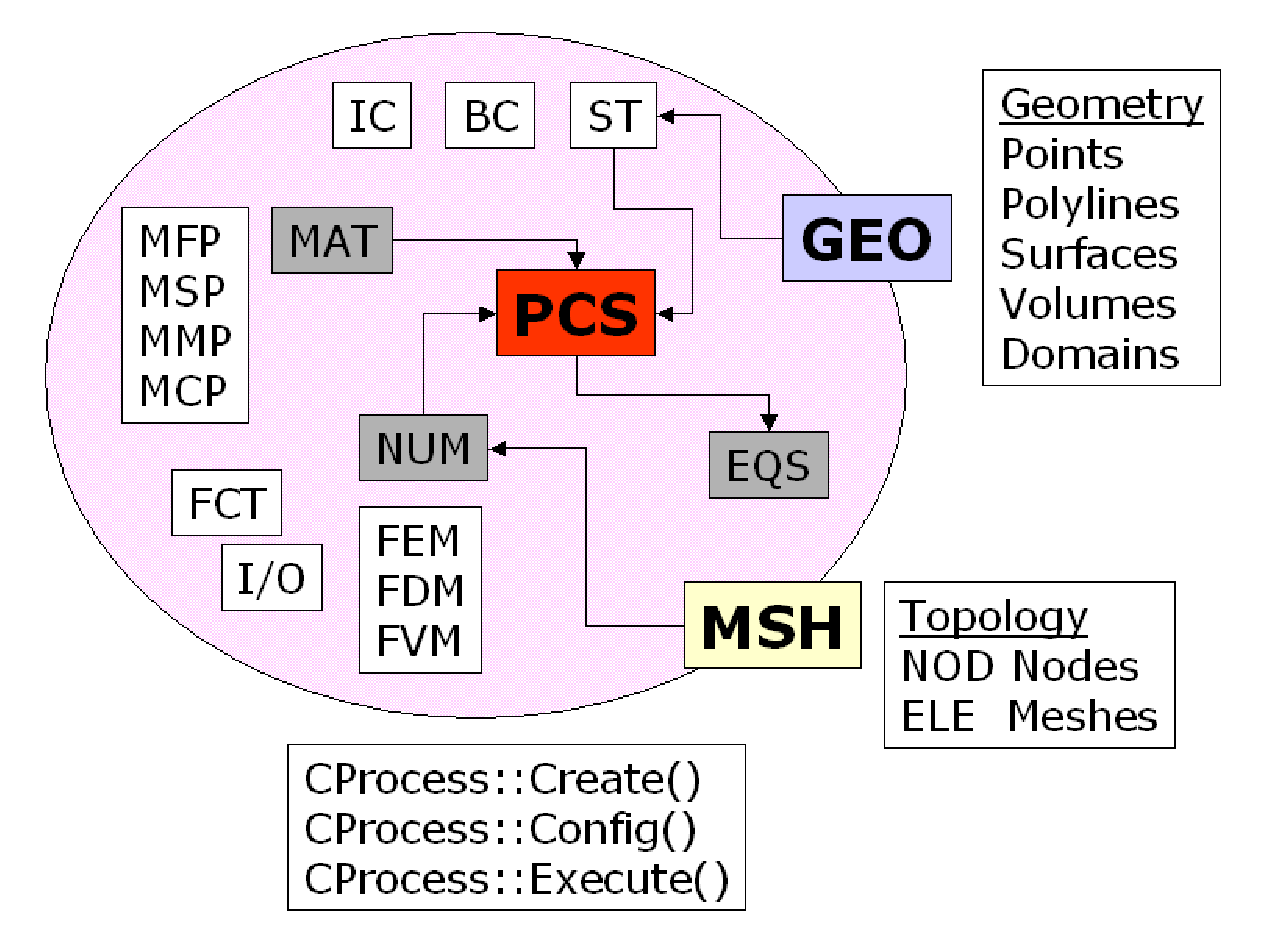
\includegraphics[scale=0.5]{figures/pcs.eps}
\caption{Structure of the process (PCS) object} \label{fig:pcs}
\end{figure}

%-------------------------------------------------------------------------
\subsection{PDE types}
\label{sec:pde}

IBVPs in porous media mechanics, such as fluid flow, mass and heat 
transport, deformation can be categorized into elliptic, parabolic, 
hyperbolic or mixed equation types.

As an example to explain the generalization of PDE types, we
illustrate the treatment of Laplace terms, which appear in flow,
transport as well as deformation processes. In Fig. \ref{fig:lap}
the evaluation of finite element matrices for Laplace terms, i.e.
$\mathbb{D}\partial^2/\partial x^2$ is given, where $\mathbb{D}$ is 
a problem-specific material tensor. The special part of diffusion 
terms is the calculation of second order space derivatives. The 
second line of the equation in Fig. \ref{fig:lap} represents the 
  numerical integration of matrix being transformated into reference coordinates. From the view point of 
object-orientation we are faced with the following operations: 
tensor coordinate transformation ($\mathbf{T}$), Jacobian 
($\mathbf{J}$), integration ($\int$) and computation of material 
properties ($\mathbb D$, e.g. diffusivity, conductivity tensor). The latter is the only problem-specific.

\begin{eqnarray}
\mathbf K_e 
&=&
\int\limits_{\Omega_e} \nabla \Sh \mathbb{D}(\nabla\Sh)^{\mathrm{T}} d\Omega \\
&=& 
\sum\limits_{gp=1}\limits^{no\_gp} \int\limits_{\Omega_r} w_{gp} 
\left[
\nabla \Sh \mathbb{D}(\nabla \Sh)^{\mathrm{T}} \mathrm{det}\ \mathbf{J} 
\right]
\vert_{gp} d\Omega
\end{eqnarray}

\begin{figure}[htb!]
\centering
\shadowbox{
\begin{minipage}{0.95\textwidth}
%{\sffamily \raggedright \small
{\ttfamily \raggedright \small
void\ CFiniteElement::CalcLaplace()\\
\{\\
\ \ \textsl{//\ Loop\ over\ Gauss\ points}\\
\ \ \textbf{for}\ (gp\ =\ 0;\ gp\ $<${}\ no\_gp;\ gp++)\\
\ \ \{\\
\mbox{\ \ \ \ \ GaussData();\ \ \ \ \ \ \ \ \ \ \ \ \ \ \ \ \ \textsl{//\ Integration\ points\ and\ weights}}\\
\mbox{\ \ \ \ \ Jacobian();\ \ \ \ \ \ \ \ \ \ \ \  \ \ \ \ \ \ \textsl{//\ det\ $\mathbf{J}$,\ ${\mathbf J}^{-1}$}}\\
\ \ \ \ \ GradShapefct();\ \ \ \ \ \  \ \ \ \ \ \ \ \ \textsl{//\ $\nabla \Sh$}\\
\mbox{\ \ \ \ \ LaplaceMATFunction();\ \ \ \ \ \ \ \ \textsl{//\ Material\ parameters,\ $\mathbb{D}$}}\\
\mbox{\ \ \ \ \ \textbf{for}\ (i=0;\ i$<${}nnodes;\ i++)\ \ \ \ \textsl{//\ Loop\ over\ element\ nodes}}\\
\ \ \ \ \ \ \ \ \textbf{for}\ (j\ =\ 0;\ j\ $<${}\ nnodes;\ j++)\\
\ \ \ \ \ \ \ \ \ \{\\
\mbox{\ \ \ \ \ \ \ \ \ \ \ \ \textbf{if}(j$>${}i)\ \textbf{continue};\ \ \ \ \textsl{//\ Symmetry}}\\
\mbox{\ \ \ \ \ \ \ \ \ \ \ \ \textbf{for}\ (k\ =\ 0;\ k\ <{}\ ele\underline\ dim;\ k++)}\\
\mbox{\ \ \ \ \ \ \ \ \ \ \ \ \ \ \ \textbf{for}(l=0;\ l<{}ele\underline\ dim;\ l++)}\\
\mbox{\ \ \ \ \ \ \ \ \ \ \ \ \ \ \ \ \ \ ($\ast$Laplace)(i,j)\ +=\ fkt\ $\ast$\ dshapefct[k$\ast$nnodes+i]\ }\\
\mbox{\ \ \ \ \ \ \ \ \ \ \ \ \ \ \ \ \ \ \ \ \ \ \ \ \ \ \ \ \ \ \ \ \ \ \ \ $\ast$\ mat[ele\underline\ dim$\ast$k+l]\ }\\
\mbox{\ \ \ \ \ \ \ \ \ \ \ \ \ \ \ \ \ \ \ \ \ \ \ \ \ \ \ \ \ \ \ \ \ \ \ \ $\ast$\ dshapefct[l$\ast$nnodes+j];}\\
\ \ \ \ \ \ \ \ \ \}\\
\ \ \}\\
\}\\
\ \\
 }
\normalfont\normalsize


\end{minipage}
}
\caption{Finite element Laplace matrix and implementation}
\label{fig:lap}
\end{figure}

\begin{figure}[htb!]
\centering
\shadowbox{
\begin{minipage}{0.75\textwidth}
{\ttfamily \raggedright \small
void\ CFiniteElementPCS::LaplaceMATFunction()\\
\{\\
\ \ \textsl{//\ Calculate\ conductivity\ tensor\ $\mathbb D$ for\ Laplacian}\\
\ \ \ \textbf{switch}(PcsType)\{\\
\ \ \ \ \ \ \textbf{case}\ L:\ \textsl{//\ Liquid\ flow}\\
\ \ \ \ \ \ \textbf{case}\ U:\ \textsl{//\ Unconfined\ flow}\\
\ \ \ \ \ \ \textbf{case}\ G:\ \textsl{//\ Gas\ flow}\\
\ \ \ \ \ \ \textbf{case}\ T:\ \textsl{//\ Two-{}phase\ flow}\\
\ \ \ \ \ \ \textbf{case}\ C:\ \textsl{//\ Componental\ flow}\\
\ \ \ \ \ \ \textbf{case}\ H:\ \textsl{//\ Heat\ transport}\\
\ \ \ \ \ \ \textbf{case}\ M:\ \textsl{//\ Mass\ transport}\\
\ \ \ \ \ \ \textbf{case}\ O:\ \textsl{//\ Overland\ flow}\\
\ \ \ \ \ \ \textbf{case}\ R:\ \textsl{//\ Richard\ flow}\\
\ \ \ \}\\
\}\\
\ \\
 }
\normalfont\normalsize


\end{minipage}
}
\caption{Implementation of process dependent material functions}
\label{fig:mat1}
\end{figure}

Fig. \ref{fig:lap} shows the implementation of the Laplace term
calculation, in which $\Omega_r$ is the domain by the reference 
element. The \texttt{CalcLaplace()} member function of the finite 
element class works for different processes with different material 
functions (Fig. \ref{fig:mat1}) and geometric element types. A short 
description is given in the table below.

\small
\begin{tabular}{|l|l|}
  \hline
  % after \\: \hline or \cline{col1-col2} \cline{col3-col4} ...
  \texttt{Code} & Description \\
  \hline
  \texttt{gp} & Gauss integration points \\
  \texttt{GaussData()} & Calculation of Gauss weights \\
  \texttt{Jacobian()} & Calculation of Jacobian determinant and inverse \\
  \texttt{GradShapeFunction()} & Calculation of shape function derivatives \\
  \texttt{LaplaceMATFunction()} & Calculation of material coefficients \\
  \texttt{(*Laplace)(i,j)} & Finite element matrix \\
  \hline
\end{tabular}
\normalsize

%-------------------------------------------------------------------------
\subsection{Element (ELE) types}
\label{sec:ele}

The basic concept we apply is that: element data, such as geometrical and topological
properties, as well as operations of elements, such as
element matrix calculations and treatment of boundary conditions,
can be generalized.

The element object is the fundamental entity in both PDE and
element types. In Fig. \ref{fig:ele_concept} the structure of the
element object is illustrated. The element has two kinds of
properties connected geometry and PDE types.

\begin{figure}[H]
\centering
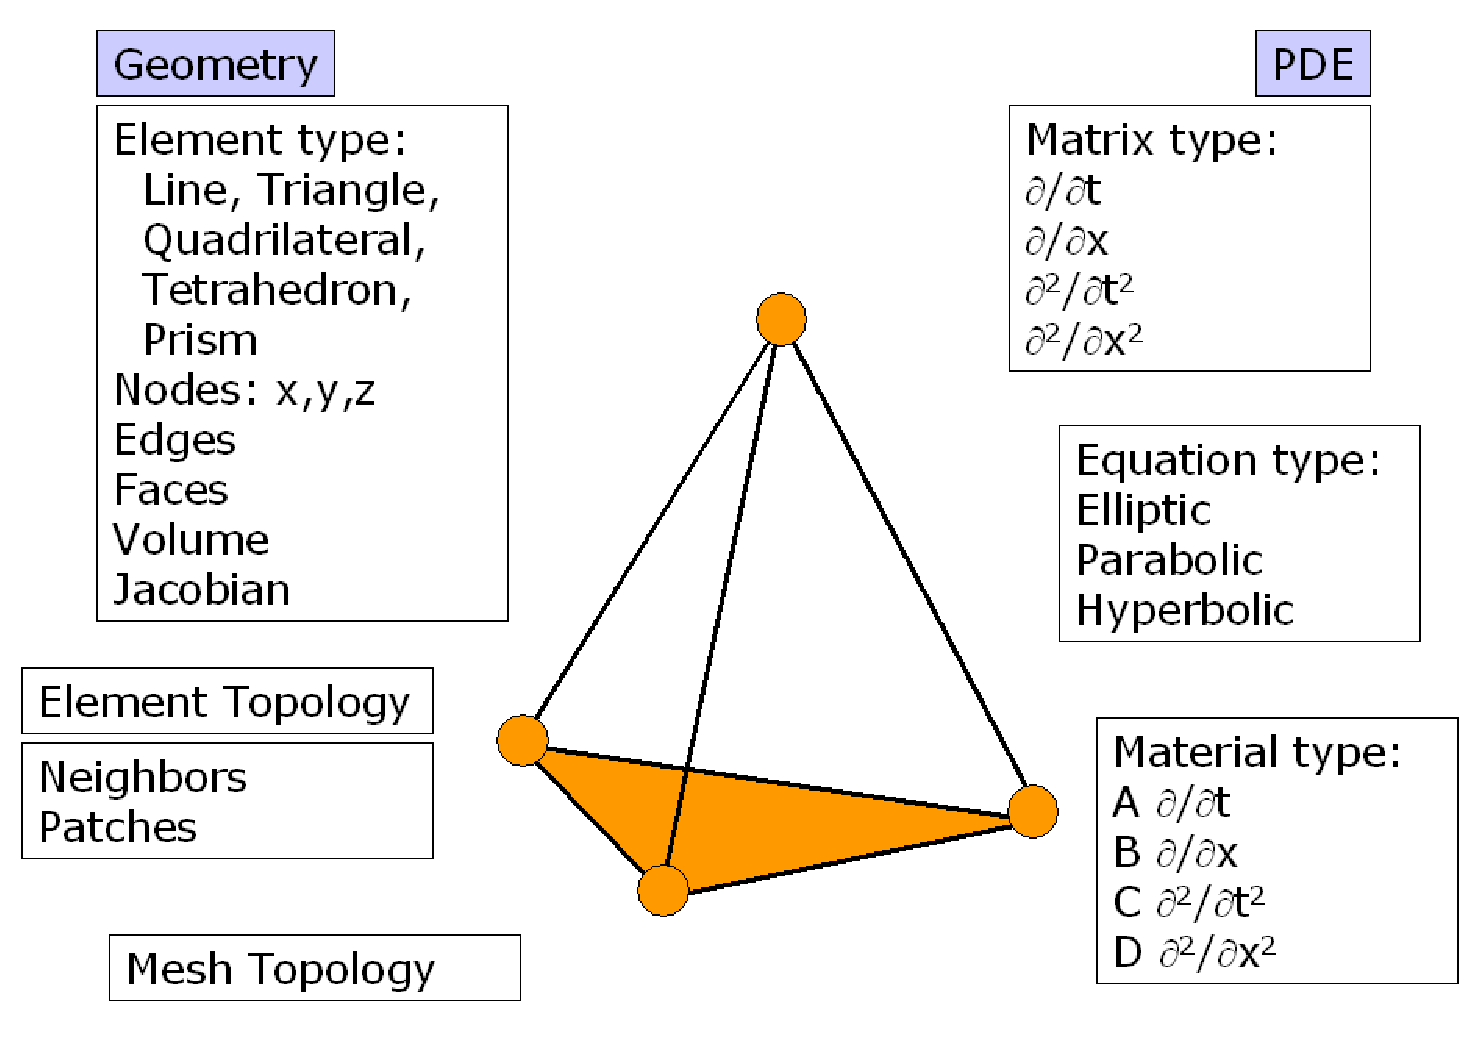
\includegraphics[scale=0.4]{figures/ele_concept.eps}
\caption{Structure of element object}
\label{fig:ele_concept}
\end{figure}

Element geometry includes the geometric type (line, triangle, quad, 
tetrahedron, prism, hexahedron), node coordinates, edges, faces and 
volume. Coordinate transformation functionalities are considered as 
geometric element properties. Element topology is defined by element 
neighbor relationships. Patch properties are available for finite 
volume approaches and flux calculations. The elements form the mesh 
topology. Different geometric element types can be combined (Fig. 
\ref{fig:ele_concept}) together to establish a mesh. Additionally, 
elements can be assigned to different meshes.
%%%% \cite{Kol:2005b}.

Depending on PDE type (elliptic, parabolic, hyperbolic, mixed),
different first or second order differential terms have to be
evaluated ($\partial/\partial t, \partial/\partial x,
\partial^2/\partial t^2, \partial^2/\partial x^2$). These differential
terms are categorized in corresponding FE matrix types (see section 
\ref{sec:fem}), mass matrix, Laplacian matrix, tangential matrix and 
coupling matrices. An obvious advantage of this element concept is 
that, depending on the geometric element type, interpolations (shape 
functions) and derivations as well as tensor operations and Gaussian 
integrations are conducted automatically in a correct way (see 
section \ref{sec:ele_fem}). For material tensor properties in 1D, 2D 
or 3D ($\mathbf{A,B,C,D(x)}$ in Fig. \ref{fig:ele_concept}), the 
correct matrix multiplications are conducted automatically. Material 
functions ($A,B,C,D(u)$ in Fig. \ref{fig:ele_concept}) are evaluated 
accordingly at corresponding Gaussian points of the selected 
element.

For the sake of object-orientation for numerical methods a so-called 
process (PCS) object was designed, implemented (\cite{KolBau:04}, 
section \ref{sec:pcs}) and successfully applied to different 
numerical methods (FEM: \cite{KolEtAl:2004a}, FDM: 
\cite{KolEtAl:2005a}, FVM: \cite{Bei:2005}).
